\documentclass[twoside]{book}

% Packages required by doxygen
\usepackage{fixltx2e}
\usepackage{calc}
\usepackage{doxygen}
\usepackage[export]{adjustbox} % also loads graphicx
\usepackage{graphicx}
\usepackage[utf8]{inputenc}
\usepackage{makeidx}
\usepackage{multicol}
\usepackage{multirow}
\PassOptionsToPackage{warn}{textcomp}
\usepackage{textcomp}
\usepackage[nointegrals]{wasysym}
\usepackage[table]{xcolor}

% Font selection
\usepackage[T1]{fontenc}
\usepackage[scaled=.90]{helvet}
\usepackage{courier}
\usepackage{amssymb}
\usepackage{sectsty}
\renewcommand{\familydefault}{\sfdefault}
\allsectionsfont{%
  \fontseries{bc}\selectfont%
  \color{darkgray}%
}
\renewcommand{\DoxyLabelFont}{%
  \fontseries{bc}\selectfont%
  \color{darkgray}%
}
\newcommand{\+}{\discretionary{\mbox{\scriptsize$\hookleftarrow$}}{}{}}

% Page & text layout
\usepackage{geometry}
\geometry{%
  a4paper,%
  top=2.5cm,%
  bottom=2.5cm,%
  left=2.5cm,%
  right=2.5cm%
}
\tolerance=750
\hfuzz=15pt
\hbadness=750
\setlength{\emergencystretch}{15pt}
\setlength{\parindent}{0cm}
\setlength{\parskip}{3ex plus 2ex minus 2ex}
\makeatletter
\renewcommand{\paragraph}{%
  \@startsection{paragraph}{4}{0ex}{-1.0ex}{1.0ex}{%
    \normalfont\normalsize\bfseries\SS@parafont%
  }%
}
\renewcommand{\subparagraph}{%
  \@startsection{subparagraph}{5}{0ex}{-1.0ex}{1.0ex}{%
    \normalfont\normalsize\bfseries\SS@subparafont%
  }%
}
\makeatother

% Headers & footers
\usepackage{fancyhdr}
\pagestyle{fancyplain}
\fancyhead[LE]{\fancyplain{}{\bfseries\thepage}}
\fancyhead[CE]{\fancyplain{}{}}
\fancyhead[RE]{\fancyplain{}{\bfseries\leftmark}}
\fancyhead[LO]{\fancyplain{}{\bfseries\rightmark}}
\fancyhead[CO]{\fancyplain{}{}}
\fancyhead[RO]{\fancyplain{}{\bfseries\thepage}}
\fancyfoot[LE]{\fancyplain{}{}}
\fancyfoot[CE]{\fancyplain{}{}}
\fancyfoot[RE]{\fancyplain{}{\bfseries\scriptsize Generated by Doxygen }}
\fancyfoot[LO]{\fancyplain{}{\bfseries\scriptsize Generated by Doxygen }}
\fancyfoot[CO]{\fancyplain{}{}}
\fancyfoot[RO]{\fancyplain{}{}}
\renewcommand{\footrulewidth}{0.4pt}
\renewcommand{\chaptermark}[1]{%
  \markboth{#1}{}%
}
\renewcommand{\sectionmark}[1]{%
  \markright{\thesection\ #1}%
}

% Indices & bibliography
\usepackage{natbib}
\usepackage[titles]{tocloft}
\setcounter{tocdepth}{3}
\setcounter{secnumdepth}{5}
\makeindex

% Hyperlinks (required, but should be loaded last)
\usepackage{ifpdf}
\ifpdf
  \usepackage[pdftex,pagebackref=true]{hyperref}
\else
  \usepackage[ps2pdf,pagebackref=true]{hyperref}
\fi
\hypersetup{%
  colorlinks=true,%
  linkcolor=blue,%
  citecolor=blue,%
  unicode%
}

% Custom commands
\newcommand{\clearemptydoublepage}{%
  \newpage{\pagestyle{empty}\cleardoublepage}%
}

\usepackage{caption}
\captionsetup{labelsep=space,justification=centering,font={bf},singlelinecheck=off,skip=4pt,position=top}

%===== C O N T E N T S =====

\begin{document}

% Titlepage & ToC
\hypersetup{pageanchor=false,
             bookmarksnumbered=true,
             pdfencoding=unicode
            }
\pagenumbering{roman}
\begin{titlepage}
\vspace*{7cm}
\begin{center}%
{\Large Path Planner A\+C\+ME Robotics }\\
\vspace*{1cm}
{\large Generated by Doxygen 1.8.11}\\
\end{center}
\end{titlepage}
\clearemptydoublepage
\tableofcontents
\clearemptydoublepage
\pagenumbering{arabic}
\hypersetup{pageanchor=true}

%--- Begin generated contents ---
\chapter{Class Index}
\section{Class List}
Here are the classes, structs, unions and interfaces with brief descriptions\+:\begin{DoxyCompactList}
\item\contentsline{section}{\hyperlink{classActions}{Actions} \\*\hyperlink{classActions}{Actions} class is used to generate movement for the robot in the action space which is in 8 directions }{\pageref{classActions}}{}
\item\contentsline{section}{\hyperlink{classAstar}{Astar} \\*\hyperlink{classAstar}{Astar} class is used to implement the A$\ast$ algorithm. Euclidean heuristic is used for this algorithm. A star gives the shortest path while avoiding obstacles }{\pageref{classAstar}}{}
\item\contentsline{section}{\hyperlink{classIksolver}{Iksolver} \\*\hyperlink{classIksolver}{Iksolver} class is used to generate the manipulator joint angles for every node generated by the path planner algorithm }{\pageref{classIksolver}}{}
\item\contentsline{section}{\hyperlink{structJointAngles}{Joint\+Angles} \\*This is a struct with six attributes which are the joint angles of the robot manipulator }{\pageref{structJointAngles}}{}
\item\contentsline{section}{\hyperlink{classMap}{Map} \\*\hyperlink{classMap}{Map} class is used to generate the map with obstacles for the A$\ast$ Algorithm and check validity of given locations }{\pageref{classMap}}{}
\item\contentsline{section}{\hyperlink{classNodesManager}{Nodes\+Manager} \\*\hyperlink{classNodesManager}{Nodes\+Manager} class is used to manage and update all the matrices that is required for implementation of A star algorithm }{\pageref{classNodesManager}}{}
\item\contentsline{section}{\hyperlink{structPosition}{Position} \\*This is a struct with two attributes x and y }{\pageref{structPosition}}{}
\end{DoxyCompactList}

\chapter{File Index}
\section{File List}
Here is a list of all documented files with brief descriptions\+:\begin{DoxyCompactList}
\item\contentsline{section}{app/\hyperlink{main_8cpp}{main.\+cpp} \\*This is the main file for this project }{\pageref{main_8cpp}}{}
\item\contentsline{section}{include/{\bfseries Actions.\+h} }{\pageref{Actions_8h}}{}
\item\contentsline{section}{include/{\bfseries Astar.\+h} }{\pageref{Astar_8h}}{}
\item\contentsline{section}{include/{\bfseries Iksolver.\+h} }{\pageref{Iksolver_8h}}{}
\item\contentsline{section}{include/{\bfseries Map.\+h} }{\pageref{Map_8h}}{}
\item\contentsline{section}{include/{\bfseries Nodes\+Manager.\+h} }{\pageref{NodesManager_8h}}{}
\end{DoxyCompactList}

\chapter{Class Documentation}
\hypertarget{classActions}{}\section{Actions Class Reference}
\label{classActions}\index{Actions@{Actions}}


\hyperlink{classActions}{Actions} class is used to generate movement for the robot in the action space which is in 8 directions.  




{\ttfamily \#include $<$Actions.\+h$>$}

\subsection*{Public Member Functions}
\begin{DoxyCompactItemize}
\item 
\hyperlink{structPosition}{Position} \hyperlink{classActions_aa89a2ec6e16b2ccbebdb3a21be930fa6}{move\+Up} (const \hyperlink{structPosition}{Position} \&current\+Pos)
\begin{DoxyCompactList}\small\item\em Gives the position which is above the current position. \end{DoxyCompactList}\item 
\hyperlink{structPosition}{Position} \hyperlink{classActions_aa52f67ef3ef76fa821e5a587f9582321}{move\+Down} (const \hyperlink{structPosition}{Position} \&current\+Pos)
\begin{DoxyCompactList}\small\item\em Gives the position which is below the current position. \end{DoxyCompactList}\item 
\hyperlink{structPosition}{Position} \hyperlink{classActions_adb21d8d86e5c11a29a0d8755253a739e}{move\+Left} (const \hyperlink{structPosition}{Position} \&current\+Pos)
\begin{DoxyCompactList}\small\item\em Gives the position which is to the left of the current position. \end{DoxyCompactList}\item 
\hyperlink{structPosition}{Position} \hyperlink{classActions_a324ac90167fc69643c7dbc2efc779387}{move\+Right} (const \hyperlink{structPosition}{Position} \&current\+Pos)
\begin{DoxyCompactList}\small\item\em Gives the position which is to the right of the current position. \end{DoxyCompactList}\item 
\hyperlink{structPosition}{Position} \hyperlink{classActions_a5d57168e20c11b1b07c7f1cbc0419284}{move\+Up\+Right} (const \hyperlink{structPosition}{Position} \&current\+Pos)
\begin{DoxyCompactList}\small\item\em Gives the position which is to the top-\/right of the current position. \end{DoxyCompactList}\item 
\hyperlink{structPosition}{Position} \hyperlink{classActions_a86b92a73287773ba08356fbb999fcc61}{move\+Up\+Left} (const \hyperlink{structPosition}{Position} \&current\+Pos)
\begin{DoxyCompactList}\small\item\em Gives the position which is to the top-\/left of the current position. \end{DoxyCompactList}\item 
\hyperlink{structPosition}{Position} \hyperlink{classActions_a01769dc63522cc613e8050c2266b0dbf}{move\+Down\+Right} (const \hyperlink{structPosition}{Position} \&current\+Pos)
\begin{DoxyCompactList}\small\item\em Gives the position which is to the down-\/left of the current position. \end{DoxyCompactList}\item 
\hyperlink{structPosition}{Position} \hyperlink{classActions_a7ff875712d63d34aeb9760672d88e05a}{move\+Down\+Left} (const \hyperlink{structPosition}{Position} \&current\+Pos)
\begin{DoxyCompactList}\small\item\em Gives the position which is to the bottom right of the current position. \end{DoxyCompactList}\end{DoxyCompactItemize}


\subsection{Detailed Description}
\hyperlink{classActions}{Actions} class is used to generate movement for the robot in the action space which is in 8 directions. 

\subsection{Member Function Documentation}
\index{Actions@{Actions}!move\+Down@{move\+Down}}
\index{move\+Down@{move\+Down}!Actions@{Actions}}
\subsubsection[{\texorpdfstring{move\+Down(const Position \&current\+Pos)}{moveDown(const Position &currentPos)}}]{\setlength{\rightskip}{0pt plus 5cm}{\bf Position} Actions\+::move\+Down (
\begin{DoxyParamCaption}
\item[{const {\bf Position} \&}]{current\+Pos}
\end{DoxyParamCaption}
)}\hypertarget{classActions_aa52f67ef3ef76fa821e5a587f9582321}{}\label{classActions_aa52f67ef3ef76fa821e5a587f9582321}


Gives the position which is below the current position. 


\begin{DoxyParams}{Parameters}
{\em \hyperlink{structPosition}{Position}} & struct which has x,y value, coordinates of a given location \\
\hline
\end{DoxyParams}
\begin{DoxyReturn}{Returns}
\hyperlink{structPosition}{Position} struct which has x,y value, coordinates of new position. 
\end{DoxyReturn}
\index{Actions@{Actions}!move\+Down\+Left@{move\+Down\+Left}}
\index{move\+Down\+Left@{move\+Down\+Left}!Actions@{Actions}}
\subsubsection[{\texorpdfstring{move\+Down\+Left(const Position \&current\+Pos)}{moveDownLeft(const Position &currentPos)}}]{\setlength{\rightskip}{0pt plus 5cm}{\bf Position} Actions\+::move\+Down\+Left (
\begin{DoxyParamCaption}
\item[{const {\bf Position} \&}]{current\+Pos}
\end{DoxyParamCaption}
)}\hypertarget{classActions_a7ff875712d63d34aeb9760672d88e05a}{}\label{classActions_a7ff875712d63d34aeb9760672d88e05a}


Gives the position which is to the bottom right of the current position. 


\begin{DoxyParams}{Parameters}
{\em \hyperlink{structPosition}{Position}} & struct which has x,y value, coordinates of a given location \\
\hline
\end{DoxyParams}
\begin{DoxyReturn}{Returns}
\hyperlink{structPosition}{Position} struct which has x,y value, coordinates of new position. 
\end{DoxyReturn}
\index{Actions@{Actions}!move\+Down\+Right@{move\+Down\+Right}}
\index{move\+Down\+Right@{move\+Down\+Right}!Actions@{Actions}}
\subsubsection[{\texorpdfstring{move\+Down\+Right(const Position \&current\+Pos)}{moveDownRight(const Position &currentPos)}}]{\setlength{\rightskip}{0pt plus 5cm}{\bf Position} Actions\+::move\+Down\+Right (
\begin{DoxyParamCaption}
\item[{const {\bf Position} \&}]{current\+Pos}
\end{DoxyParamCaption}
)}\hypertarget{classActions_a01769dc63522cc613e8050c2266b0dbf}{}\label{classActions_a01769dc63522cc613e8050c2266b0dbf}


Gives the position which is to the down-\/left of the current position. 


\begin{DoxyParams}{Parameters}
{\em \hyperlink{structPosition}{Position}} & struct which has x,y value, coordinates of a given location \\
\hline
\end{DoxyParams}
\begin{DoxyReturn}{Returns}
\hyperlink{structPosition}{Position} struct which has x,y value, coordinates of new position. 
\end{DoxyReturn}
\index{Actions@{Actions}!move\+Left@{move\+Left}}
\index{move\+Left@{move\+Left}!Actions@{Actions}}
\subsubsection[{\texorpdfstring{move\+Left(const Position \&current\+Pos)}{moveLeft(const Position &currentPos)}}]{\setlength{\rightskip}{0pt plus 5cm}{\bf Position} Actions\+::move\+Left (
\begin{DoxyParamCaption}
\item[{const {\bf Position} \&}]{current\+Pos}
\end{DoxyParamCaption}
)}\hypertarget{classActions_adb21d8d86e5c11a29a0d8755253a739e}{}\label{classActions_adb21d8d86e5c11a29a0d8755253a739e}


Gives the position which is to the left of the current position. 


\begin{DoxyParams}{Parameters}
{\em \hyperlink{structPosition}{Position}} & struct which has x,y value, coordinates of a given location \\
\hline
\end{DoxyParams}
\begin{DoxyReturn}{Returns}
\hyperlink{structPosition}{Position} struct which has x,y value, coordinates of new position. 
\end{DoxyReturn}
\index{Actions@{Actions}!move\+Right@{move\+Right}}
\index{move\+Right@{move\+Right}!Actions@{Actions}}
\subsubsection[{\texorpdfstring{move\+Right(const Position \&current\+Pos)}{moveRight(const Position &currentPos)}}]{\setlength{\rightskip}{0pt plus 5cm}{\bf Position} Actions\+::move\+Right (
\begin{DoxyParamCaption}
\item[{const {\bf Position} \&}]{current\+Pos}
\end{DoxyParamCaption}
)}\hypertarget{classActions_a324ac90167fc69643c7dbc2efc779387}{}\label{classActions_a324ac90167fc69643c7dbc2efc779387}


Gives the position which is to the right of the current position. 


\begin{DoxyParams}{Parameters}
{\em \hyperlink{structPosition}{Position}} & struct which has x,y value, coordinates of a given location \\
\hline
\end{DoxyParams}
\begin{DoxyReturn}{Returns}
\hyperlink{structPosition}{Position} struct which has x,y value, coordinates of new position. 
\end{DoxyReturn}
\index{Actions@{Actions}!move\+Up@{move\+Up}}
\index{move\+Up@{move\+Up}!Actions@{Actions}}
\subsubsection[{\texorpdfstring{move\+Up(const Position \&current\+Pos)}{moveUp(const Position &currentPos)}}]{\setlength{\rightskip}{0pt plus 5cm}{\bf Position} Actions\+::move\+Up (
\begin{DoxyParamCaption}
\item[{const {\bf Position} \&}]{current\+Pos}
\end{DoxyParamCaption}
)}\hypertarget{classActions_aa89a2ec6e16b2ccbebdb3a21be930fa6}{}\label{classActions_aa89a2ec6e16b2ccbebdb3a21be930fa6}


Gives the position which is above the current position. 


\begin{DoxyParams}{Parameters}
{\em \hyperlink{structPosition}{Position}} & struct which has x,y value, coordinates of a given location \\
\hline
\end{DoxyParams}
\begin{DoxyReturn}{Returns}
\hyperlink{structPosition}{Position} struct which has x,y value, coordinates of new position. 
\end{DoxyReturn}
\index{Actions@{Actions}!move\+Up\+Left@{move\+Up\+Left}}
\index{move\+Up\+Left@{move\+Up\+Left}!Actions@{Actions}}
\subsubsection[{\texorpdfstring{move\+Up\+Left(const Position \&current\+Pos)}{moveUpLeft(const Position &currentPos)}}]{\setlength{\rightskip}{0pt plus 5cm}{\bf Position} Actions\+::move\+Up\+Left (
\begin{DoxyParamCaption}
\item[{const {\bf Position} \&}]{current\+Pos}
\end{DoxyParamCaption}
)}\hypertarget{classActions_a86b92a73287773ba08356fbb999fcc61}{}\label{classActions_a86b92a73287773ba08356fbb999fcc61}


Gives the position which is to the top-\/left of the current position. 


\begin{DoxyParams}{Parameters}
{\em \hyperlink{structPosition}{Position}} & struct which has x,y value, coordinates of a given location \\
\hline
\end{DoxyParams}
\begin{DoxyReturn}{Returns}
\hyperlink{structPosition}{Position} struct which has x,y value, coordinates of new position. 
\end{DoxyReturn}
\index{Actions@{Actions}!move\+Up\+Right@{move\+Up\+Right}}
\index{move\+Up\+Right@{move\+Up\+Right}!Actions@{Actions}}
\subsubsection[{\texorpdfstring{move\+Up\+Right(const Position \&current\+Pos)}{moveUpRight(const Position &currentPos)}}]{\setlength{\rightskip}{0pt plus 5cm}{\bf Position} Actions\+::move\+Up\+Right (
\begin{DoxyParamCaption}
\item[{const {\bf Position} \&}]{current\+Pos}
\end{DoxyParamCaption}
)}\hypertarget{classActions_a5d57168e20c11b1b07c7f1cbc0419284}{}\label{classActions_a5d57168e20c11b1b07c7f1cbc0419284}


Gives the position which is to the top-\/right of the current position. 


\begin{DoxyParams}{Parameters}
{\em \hyperlink{structPosition}{Position}} & struct which has x,y value, coordinates of a given location \\
\hline
\end{DoxyParams}
\begin{DoxyReturn}{Returns}
\hyperlink{structPosition}{Position} struct which has x,y value, coordinates of new position. 
\end{DoxyReturn}


The documentation for this class was generated from the following files\+:\begin{DoxyCompactItemize}
\item 
include/Actions.\+h\item 
app/Actions.\+cpp\end{DoxyCompactItemize}

\hypertarget{classAstar}{}\section{Astar Class Reference}
\label{classAstar}\index{Astar@{Astar}}


\hyperlink{classAstar}{Astar} class is used to implement the A$\ast$ algorithm. Euclidean heuristic is used for this algorithm. A star gives the shortest path while avoiding obstacles.  




{\ttfamily \#include $<$Astar.\+h$>$}

\subsection*{Public Member Functions}
\begin{DoxyCompactItemize}
\item 
\hyperlink{classAstar_a9f5d925a6e411e851234ab4ef311e7f7}{Astar} (\hyperlink{classMap}{Map} \&map)
\item 
std\+::vector$<$ Eigen\+::\+Vector2d $>$ \hyperlink{classAstar_a4addd7a1866da125d6bb035e52f08627}{a\+Star\+Algorithm} ()
\begin{DoxyCompactList}\small\item\em In this method, the shortest path will be computed using the A$\ast$ algorithm. \end{DoxyCompactList}\item 
void \hyperlink{classAstar_a71dab0041f5937321717a503d3aa1827}{path\+Backtracking} ()
\begin{DoxyCompactList}\small\item\em shows the final path which was computed by the A$\ast$ algorithm (Backtracking) \end{DoxyCompactList}\item 
void \hyperlink{classAstar_a47ad9c479ad2a824d5902bd76d8fd88a}{check\+And\+Update} (const \hyperlink{structPosition}{Position} \&current\+Position, const \hyperlink{structPosition}{Position} \&new\+Position, double d)
\item 
double \hyperlink{classAstar_a489c224e6100635858f738a64d408e0e}{compute\+Cost\+To\+Go} (const \hyperlink{structPosition}{Position} \&pos)
\begin{DoxyCompactList}\small\item\em Calculates the cost to go for the current position and goal position (Euclidean Distance between the two points) \end{DoxyCompactList}\item 
\hyperlink{structPosition}{Position} \hyperlink{classAstar_a4acb8dce728cdd0b296c7069e96143e3}{get\+Start\+Position} ()
\begin{DoxyCompactList}\small\item\em Is used to retrieve the start position. \end{DoxyCompactList}\item 
\hyperlink{structPosition}{Position} \hyperlink{classAstar_ad833c2038e84c544e3bdf22657663346}{get\+Goal\+Position} ()
\begin{DoxyCompactList}\small\item\em Is used to retrieve the goal position. \end{DoxyCompactList}\item 
void \hyperlink{classAstar_ab2f62826b10ad7fe479948bca50b27b7}{set\+Start\+Position} (int x, int y)
\begin{DoxyCompactList}\small\item\em Is used to set the start position. \end{DoxyCompactList}\item 
void \hyperlink{classAstar_a23c5c0f315830d742382562319b250c6}{set\+Goal\+Position} (int x, int y)
\begin{DoxyCompactList}\small\item\em Is used to set the goal position. \end{DoxyCompactList}\end{DoxyCompactItemize}


\subsection{Detailed Description}
\hyperlink{classAstar}{Astar} class is used to implement the A$\ast$ algorithm. Euclidean heuristic is used for this algorithm. A star gives the shortest path while avoiding obstacles. 

\subsection{Constructor \& Destructor Documentation}
\index{Astar@{Astar}!Astar@{Astar}}
\index{Astar@{Astar}!Astar@{Astar}}
\subsubsection[{\texorpdfstring{Astar(\+Map \&map)}{Astar(Map &map)}}]{\setlength{\rightskip}{0pt plus 5cm}Astar\+::\+Astar (
\begin{DoxyParamCaption}
\item[{{\bf Map} \&}]{map}
\end{DoxyParamCaption}
)\hspace{0.3cm}{\ttfamily [explicit]}}\hypertarget{classAstar_a9f5d925a6e411e851234ab4ef311e7f7}{}\label{classAstar_a9f5d925a6e411e851234ab4ef311e7f7}
one argument constructor that takes object of class map by reference. 

\subsection{Member Function Documentation}
\index{Astar@{Astar}!a\+Star\+Algorithm@{a\+Star\+Algorithm}}
\index{a\+Star\+Algorithm@{a\+Star\+Algorithm}!Astar@{Astar}}
\subsubsection[{\texorpdfstring{a\+Star\+Algorithm()}{aStarAlgorithm()}}]{\setlength{\rightskip}{0pt plus 5cm}std\+::vector$<$ Eigen\+::\+Vector2d $>$ Astar\+::a\+Star\+Algorithm (
\begin{DoxyParamCaption}
{}
\end{DoxyParamCaption}
)}\hypertarget{classAstar_a4addd7a1866da125d6bb035e52f08627}{}\label{classAstar_a4addd7a1866da125d6bb035e52f08627}


In this method, the shortest path will be computed using the A$\ast$ algorithm. 


\begin{DoxyParams}{Parameters}
{\em None} & \\
\hline
\end{DoxyParams}
\begin{DoxyReturn}{Returns}
std\+::vector$<$\+Eigen\+::\+Vector2d$>$ returns path obtained from astar algorithm. 
\end{DoxyReturn}
\index{Astar@{Astar}!check\+And\+Update@{check\+And\+Update}}
\index{check\+And\+Update@{check\+And\+Update}!Astar@{Astar}}
\subsubsection[{\texorpdfstring{check\+And\+Update(const Position \&current\+Position, const Position \&new\+Position, double d)}{checkAndUpdate(const Position &currentPosition, const Position &newPosition, double d)}}]{\setlength{\rightskip}{0pt plus 5cm}void Astar\+::check\+And\+Update (
\begin{DoxyParamCaption}
\item[{const {\bf Position} \&}]{current\+Position, }
\item[{const {\bf Position} \&}]{new\+Position, }
\item[{double}]{d}
\end{DoxyParamCaption}
)}\hypertarget{classAstar_a47ad9c479ad2a824d5902bd76d8fd88a}{}\label{classAstar_a47ad9c479ad2a824d5902bd76d8fd88a}

\begin{DoxyParams}{Parameters}
{\em struct} & position that represents current position of the robot on the map. \\
\hline
{\em struct} & new position that represents next position of the robot on the map \\
\hline
{\em double} & d which specifies cost specific to an action 1 for up down right left. sqrt(2) for remaining four actions. \\
\hline
\end{DoxyParams}
\begin{DoxyReturn}{Returns}
None 
\end{DoxyReturn}
\index{Astar@{Astar}!compute\+Cost\+To\+Go@{compute\+Cost\+To\+Go}}
\index{compute\+Cost\+To\+Go@{compute\+Cost\+To\+Go}!Astar@{Astar}}
\subsubsection[{\texorpdfstring{compute\+Cost\+To\+Go(const Position \&pos)}{computeCostToGo(const Position &pos)}}]{\setlength{\rightskip}{0pt plus 5cm}double Astar\+::compute\+Cost\+To\+Go (
\begin{DoxyParamCaption}
\item[{const {\bf Position} \&}]{pos}
\end{DoxyParamCaption}
)}\hypertarget{classAstar_a489c224e6100635858f738a64d408e0e}{}\label{classAstar_a489c224e6100635858f738a64d408e0e}


Calculates the cost to go for the current position and goal position (Euclidean Distance between the two points) 


\begin{DoxyParams}{Parameters}
{\em current} & position, stuct \hyperlink{structPosition}{Position} \\
\hline
\end{DoxyParams}
\begin{DoxyReturn}{Returns}
Double Cost to go 
\end{DoxyReturn}
\index{Astar@{Astar}!get\+Goal\+Position@{get\+Goal\+Position}}
\index{get\+Goal\+Position@{get\+Goal\+Position}!Astar@{Astar}}
\subsubsection[{\texorpdfstring{get\+Goal\+Position()}{getGoalPosition()}}]{\setlength{\rightskip}{0pt plus 5cm}{\bf Position} Astar\+::get\+Goal\+Position (
\begin{DoxyParamCaption}
{}
\end{DoxyParamCaption}
)}\hypertarget{classAstar_ad833c2038e84c544e3bdf22657663346}{}\label{classAstar_ad833c2038e84c544e3bdf22657663346}


Is used to retrieve the goal position. 


\begin{DoxyParams}{Parameters}
{\em None} & \\
\hline
\end{DoxyParams}
\begin{DoxyReturn}{Returns}
Struct position 
\end{DoxyReturn}
\index{Astar@{Astar}!get\+Start\+Position@{get\+Start\+Position}}
\index{get\+Start\+Position@{get\+Start\+Position}!Astar@{Astar}}
\subsubsection[{\texorpdfstring{get\+Start\+Position()}{getStartPosition()}}]{\setlength{\rightskip}{0pt plus 5cm}{\bf Position} Astar\+::get\+Start\+Position (
\begin{DoxyParamCaption}
{}
\end{DoxyParamCaption}
)}\hypertarget{classAstar_a4acb8dce728cdd0b296c7069e96143e3}{}\label{classAstar_a4acb8dce728cdd0b296c7069e96143e3}


Is used to retrieve the start position. 


\begin{DoxyParams}{Parameters}
{\em None} & \\
\hline
\end{DoxyParams}
\begin{DoxyReturn}{Returns}
Struct position 
\end{DoxyReturn}
\index{Astar@{Astar}!path\+Backtracking@{path\+Backtracking}}
\index{path\+Backtracking@{path\+Backtracking}!Astar@{Astar}}
\subsubsection[{\texorpdfstring{path\+Backtracking()}{pathBacktracking()}}]{\setlength{\rightskip}{0pt plus 5cm}void Astar\+::path\+Backtracking (
\begin{DoxyParamCaption}
{}
\end{DoxyParamCaption}
)}\hypertarget{classAstar_a71dab0041f5937321717a503d3aa1827}{}\label{classAstar_a71dab0041f5937321717a503d3aa1827}


shows the final path which was computed by the A$\ast$ algorithm (Backtracking) 


\begin{DoxyParams}{Parameters}
{\em None} & \\
\hline
\end{DoxyParams}
\begin{DoxyReturn}{Returns}
None 
\end{DoxyReturn}
\index{Astar@{Astar}!set\+Goal\+Position@{set\+Goal\+Position}}
\index{set\+Goal\+Position@{set\+Goal\+Position}!Astar@{Astar}}
\subsubsection[{\texorpdfstring{set\+Goal\+Position(int x, int y)}{setGoalPosition(int x, int y)}}]{\setlength{\rightskip}{0pt plus 5cm}void Astar\+::set\+Goal\+Position (
\begin{DoxyParamCaption}
\item[{int}]{x, }
\item[{int}]{y}
\end{DoxyParamCaption}
)}\hypertarget{classAstar_a23c5c0f315830d742382562319b250c6}{}\label{classAstar_a23c5c0f315830d742382562319b250c6}


Is used to set the goal position. 


\begin{DoxyParams}{Parameters}
{\em int} & x and y coordinates for goal position \\
\hline
\end{DoxyParams}
\begin{DoxyReturn}{Returns}
None 
\end{DoxyReturn}
\index{Astar@{Astar}!set\+Start\+Position@{set\+Start\+Position}}
\index{set\+Start\+Position@{set\+Start\+Position}!Astar@{Astar}}
\subsubsection[{\texorpdfstring{set\+Start\+Position(int x, int y)}{setStartPosition(int x, int y)}}]{\setlength{\rightskip}{0pt plus 5cm}void Astar\+::set\+Start\+Position (
\begin{DoxyParamCaption}
\item[{int}]{x, }
\item[{int}]{y}
\end{DoxyParamCaption}
)}\hypertarget{classAstar_ab2f62826b10ad7fe479948bca50b27b7}{}\label{classAstar_ab2f62826b10ad7fe479948bca50b27b7}


Is used to set the start position. 


\begin{DoxyParams}{Parameters}
{\em int} & x and y coordinates for start position \\
\hline
\end{DoxyParams}
\begin{DoxyReturn}{Returns}
None 
\end{DoxyReturn}


The documentation for this class was generated from the following files\+:\begin{DoxyCompactItemize}
\item 
include/Astar.\+h\item 
app/Astar.\+cpp\end{DoxyCompactItemize}

\hypertarget{classIksolver}{}\section{Iksolver Class Reference}
\label{classIksolver}\index{Iksolver@{Iksolver}}


\hyperlink{classIksolver}{Iksolver} class is used to generate the manipulator joint angles for every node generated by the path planner algorithm.  




{\ttfamily \#include $<$Iksolver.\+h$>$}

\subsection*{Public Member Functions}
\begin{DoxyCompactItemize}
\item 
std\+::vector$<$ \hyperlink{structJointAngles}{Joint\+Angles} $>$ \hyperlink{classIksolver_a008092b5e02014fc1dcd904ae085de37}{ik\+Solver} (std\+::vector$<$ Eigen\+::\+Vector2d $>$ path)
\begin{DoxyCompactList}\small\item\em This function is used to display the set of 6 joint angles of manipulator(6 dof arm) for every point in the path computed from the A star algorithm. \end{DoxyCompactList}\end{DoxyCompactItemize}


\subsection{Detailed Description}
\hyperlink{classIksolver}{Iksolver} class is used to generate the manipulator joint angles for every node generated by the path planner algorithm. 

\subsection{Member Function Documentation}
\index{Iksolver@{Iksolver}!ik\+Solver@{ik\+Solver}}
\index{ik\+Solver@{ik\+Solver}!Iksolver@{Iksolver}}
\subsubsection[{\texorpdfstring{ik\+Solver(std\+::vector$<$ Eigen\+::\+Vector2d $>$ path)}{ikSolver(std::vector< Eigen::Vector2d > path)}}]{\setlength{\rightskip}{0pt plus 5cm}std\+::vector$<$ {\bf Joint\+Angles} $>$ Iksolver\+::ik\+Solver (
\begin{DoxyParamCaption}
\item[{std\+::vector$<$ Eigen\+::\+Vector2d $>$}]{path}
\end{DoxyParamCaption}
)}\hypertarget{classIksolver_a008092b5e02014fc1dcd904ae085de37}{}\label{classIksolver_a008092b5e02014fc1dcd904ae085de37}


This function is used to display the set of 6 joint angles of manipulator(6 dof arm) for every point in the path computed from the A star algorithm. 


\begin{DoxyParams}{Parameters}
{\em path,which} & is the output from A$\ast$star algorithm i.\+e. the shortest path between start and goal points \\
\hline
\end{DoxyParams}
\begin{DoxyReturn}{Returns}
a vector containing struct of joint angles. 
\end{DoxyReturn}


The documentation for this class was generated from the following files\+:\begin{DoxyCompactItemize}
\item 
include/Iksolver.\+h\item 
app/Iksolver.\+cpp\end{DoxyCompactItemize}

\hypertarget{structJointAngles}{}\section{Joint\+Angles Struct Reference}
\label{structJointAngles}\index{Joint\+Angles@{Joint\+Angles}}


This is a struct with six attributes which are the joint angles of the robot manipulator.  




{\ttfamily \#include $<$Iksolver.\+h$>$}

\subsection*{Public Attributes}
\begin{DoxyCompactItemize}
\item 
double {\bfseries thetha1} = 10\hypertarget{structJointAngles_a25ef8e13ef8babc95e27fb7004692f9a}{}\label{structJointAngles_a25ef8e13ef8babc95e27fb7004692f9a}

\item 
double {\bfseries thetha2} = 10\hypertarget{structJointAngles_acf0d666376d537675ab8f093e4e0676e}{}\label{structJointAngles_acf0d666376d537675ab8f093e4e0676e}

\item 
double {\bfseries thetha3} = 10\hypertarget{structJointAngles_ab6e6bd7a72a2c5c15e09823f717eda82}{}\label{structJointAngles_ab6e6bd7a72a2c5c15e09823f717eda82}

\item 
double {\bfseries thetha4} = 10\hypertarget{structJointAngles_af5b00557e096dd9f21d4038dd4b008ba}{}\label{structJointAngles_af5b00557e096dd9f21d4038dd4b008ba}

\item 
double {\bfseries thetha5} = 10\hypertarget{structJointAngles_ace9588d1858f90e2f31afde1e05aece4}{}\label{structJointAngles_ace9588d1858f90e2f31afde1e05aece4}

\item 
double {\bfseries thetha6} = 10\hypertarget{structJointAngles_a3a3ed376b7354d1def6fd5ea7d909c67}{}\label{structJointAngles_a3a3ed376b7354d1def6fd5ea7d909c67}

\end{DoxyCompactItemize}


\subsection{Detailed Description}
This is a struct with six attributes which are the joint angles of the robot manipulator. 

The documentation for this struct was generated from the following file\+:\begin{DoxyCompactItemize}
\item 
include/Iksolver.\+h\end{DoxyCompactItemize}

\hypertarget{classMap}{}\section{Map Class Reference}
\label{classMap}\index{Map@{Map}}


\hyperlink{classMap}{Map} class is used to generate the map with obstacles for the A$\ast$ Algorithm and check validity of given locations.  




{\ttfamily \#include $<$Map.\+h$>$}

\subsection*{Public Member Functions}
\begin{DoxyCompactItemize}
\item 
bool \hyperlink{classMap_af39ac88e2c0f961c60e95b3f7dd00602}{obstacle\+Check} (const \hyperlink{structPosition}{Position} \&new\+Pos)
\begin{DoxyCompactList}\small\item\em Checks presence of obstacle at the given location where obstacle is represented by \textquotesingle{}1\textquotesingle{} and workspace is represented by \textquotesingle{}0\textquotesingle{} in the map. \end{DoxyCompactList}\item 
bool \hyperlink{classMap_a4d4d1d84c2888a7233cf9174b45c0a11}{validity\+Check} (const \hyperlink{structPosition}{Position} \&new\+Pos)
\begin{DoxyCompactList}\small\item\em Checks validity of the given location i.\+e. if the point lies within the bounds of the map. \end{DoxyCompactList}\item 
void \hyperlink{classMap_a6882934f9d1877bca051a212ee3f754c}{plot\+Map} ()
\begin{DoxyCompactList}\small\item\em Displays complete map with obstacles represented by 1,0 for valid points. \end{DoxyCompactList}\item 
void \hyperlink{classMap_ab01b5945ae722908864a3208939928d1}{create\+Map} ()
\begin{DoxyCompactList}\small\item\em Creates obstacles on the map. \end{DoxyCompactList}\item 
void \hyperlink{classMap_ade005914937328a33141f3aa0e121bec}{set\+Path} (std\+::vector$<$ Eigen\+::\+Vector2d $>$ path)
\end{DoxyCompactItemize}


\subsection{Detailed Description}
\hyperlink{classMap}{Map} class is used to generate the map with obstacles for the A$\ast$ Algorithm and check validity of given locations. 

\subsection{Member Function Documentation}
\index{Map@{Map}!create\+Map@{create\+Map}}
\index{create\+Map@{create\+Map}!Map@{Map}}
\subsubsection[{\texorpdfstring{create\+Map()}{createMap()}}]{\setlength{\rightskip}{0pt plus 5cm}void Map\+::create\+Map (
\begin{DoxyParamCaption}
{}
\end{DoxyParamCaption}
)}\hypertarget{classMap_ab01b5945ae722908864a3208939928d1}{}\label{classMap_ab01b5945ae722908864a3208939928d1}


Creates obstacles on the map. 


\begin{DoxyParams}{Parameters}
{\em None} & \\
\hline
\end{DoxyParams}
\begin{DoxyReturn}{Returns}
None 
\end{DoxyReturn}
\index{Map@{Map}!obstacle\+Check@{obstacle\+Check}}
\index{obstacle\+Check@{obstacle\+Check}!Map@{Map}}
\subsubsection[{\texorpdfstring{obstacle\+Check(const Position \&new\+Pos)}{obstacleCheck(const Position &newPos)}}]{\setlength{\rightskip}{0pt plus 5cm}bool Map\+::obstacle\+Check (
\begin{DoxyParamCaption}
\item[{const {\bf Position} \&}]{new\+Pos}
\end{DoxyParamCaption}
)}\hypertarget{classMap_af39ac88e2c0f961c60e95b3f7dd00602}{}\label{classMap_af39ac88e2c0f961c60e95b3f7dd00602}


Checks presence of obstacle at the given location where obstacle is represented by \textquotesingle{}1\textquotesingle{} and workspace is represented by \textquotesingle{}0\textquotesingle{} in the map. 


\begin{DoxyParams}{Parameters}
{\em \hyperlink{structPosition}{Position}} & struct which has x,y value, coordinates of a given location. \\
\hline
\end{DoxyParams}
\begin{DoxyReturn}{Returns}
Boolean returns true if there is obstacle, false otherwise. 
\end{DoxyReturn}
\index{Map@{Map}!plot\+Map@{plot\+Map}}
\index{plot\+Map@{plot\+Map}!Map@{Map}}
\subsubsection[{\texorpdfstring{plot\+Map()}{plotMap()}}]{\setlength{\rightskip}{0pt plus 5cm}void Map\+::plot\+Map (
\begin{DoxyParamCaption}
{}
\end{DoxyParamCaption}
)}\hypertarget{classMap_a6882934f9d1877bca051a212ee3f754c}{}\label{classMap_a6882934f9d1877bca051a212ee3f754c}


Displays complete map with obstacles represented by 1,0 for valid points. 


\begin{DoxyParams}{Parameters}
{\em None} & \\
\hline
\end{DoxyParams}
\begin{DoxyReturn}{Returns}
None 
\end{DoxyReturn}
\index{Map@{Map}!set\+Path@{set\+Path}}
\index{set\+Path@{set\+Path}!Map@{Map}}
\subsubsection[{\texorpdfstring{set\+Path(std\+::vector$<$ Eigen\+::\+Vector2d $>$ path)}{setPath(std::vector< Eigen::Vector2d > path)}}]{\setlength{\rightskip}{0pt plus 5cm}void Map\+::set\+Path (
\begin{DoxyParamCaption}
\item[{std\+::vector$<$ Eigen\+::\+Vector2d $>$}]{path}
\end{DoxyParamCaption}
)}\hypertarget{classMap_ade005914937328a33141f3aa0e121bec}{}\label{classMap_ade005914937328a33141f3aa0e121bec}
brief Sets the path traced by the robot by digit 5 in the matrix. 
\begin{DoxyParams}{Parameters}
{\em path} & is a vector containing the points in the form of eigen vector traced by the robot. \\
\hline
\end{DoxyParams}
\begin{DoxyReturn}{Returns}
None 
\end{DoxyReturn}
\index{Map@{Map}!validity\+Check@{validity\+Check}}
\index{validity\+Check@{validity\+Check}!Map@{Map}}
\subsubsection[{\texorpdfstring{validity\+Check(const Position \&new\+Pos)}{validityCheck(const Position &newPos)}}]{\setlength{\rightskip}{0pt plus 5cm}bool Map\+::validity\+Check (
\begin{DoxyParamCaption}
\item[{const {\bf Position} \&}]{new\+Pos}
\end{DoxyParamCaption}
)}\hypertarget{classMap_a4d4d1d84c2888a7233cf9174b45c0a11}{}\label{classMap_a4d4d1d84c2888a7233cf9174b45c0a11}


Checks validity of the given location i.\+e. if the point lies within the bounds of the map. 


\begin{DoxyParams}{Parameters}
{\em \hyperlink{structPosition}{Position}} & struct which has x,y value, coordinates of a given location. \\
\hline
\end{DoxyParams}
\begin{DoxyReturn}{Returns}
Boolean returns true if the location is valid, false otherwise. 
\end{DoxyReturn}


The documentation for this class was generated from the following files\+:\begin{DoxyCompactItemize}
\item 
include/Map.\+h\item 
app/Map.\+cpp\end{DoxyCompactItemize}

\hypertarget{classNodesManager}{}\section{Nodes\+Manager Class Reference}
\label{classNodesManager}\index{Nodes\+Manager@{Nodes\+Manager}}


\hyperlink{classNodesManager}{Nodes\+Manager} class is used to manage and update all the matrices that is required for implementation of A star algorithm.  




{\ttfamily \#include $<$Nodes\+Manager.\+h$>$}

\subsection*{Public Member Functions}
\begin{DoxyCompactItemize}
\item 
void \hyperlink{classNodesManager_af14624200c5dba19deb48628fdb38338}{update\+Visited} (const \hyperlink{structPosition}{Position} \&pos)
\begin{DoxyCompactList}\small\item\em Takes the current node as index for the Visited matrix and updates the status at that index. Status is 1 if visited, else 0. \end{DoxyCompactList}\item 
void \hyperlink{classNodesManager_a7e33a29ae5bb0fdbf061cf71cad10161}{update\+Parent} (const \hyperlink{structPosition}{Position} \&pos, int parent\+Id)
\begin{DoxyCompactList}\small\item\em Takes the current node as index for the Parent matrix and updates the parent for the node Each parent for current node is associated with unique ID. Ex. For node (1,1), (1,2) as parent. Parent for (1,1) is represented by (x-\/coordinate$\ast$100 + y-\/coordinate) i.\+e. (1,2) -\/ id is 102. \end{DoxyCompactList}\item 
void \hyperlink{classNodesManager_a97a3abf51b1a265aff8b2b0428e021bd}{update\+Cost} (const \hyperlink{structPosition}{Position} \&pos, double cost)
\begin{DoxyCompactList}\small\item\em Takes the current node as index for the Cost matrix and updates the cost at that index. \end{DoxyCompactList}\item 
void \hyperlink{classNodesManager_afe93611a7771f10bc2d6a33a01cdb80c}{update\+Cost\+To\+Come} (const \hyperlink{structPosition}{Position} \&pos, double cost)
\begin{DoxyCompactList}\small\item\em Takes the current node as index for the Cost\+To\+Come matrix and updates the cost Status is 1 if visited, else 0. \end{DoxyCompactList}\item 
void \hyperlink{classNodesManager_acb8c01841ac88537ccfaf5cafec0be26}{update\+Cost\+To\+Go} (const \hyperlink{structPosition}{Position} \&pos, double cost)
\begin{DoxyCompactList}\small\item\em Takes the current node as index for the Cost\+To\+Go matrix and updates the status Status is 1 if visited, else 0. \end{DoxyCompactList}\item 
int \hyperlink{classNodesManager_a27495b9f67db0f9955945269657b3191}{get\+Parent} (const \hyperlink{structPosition}{Position} \&pos)
\begin{DoxyCompactList}\small\item\em Returns the parent for the current node taking the current node as index in the Parent matrix. \end{DoxyCompactList}\item 
int \hyperlink{classNodesManager_a37e0acde250e53d0be293d0cdea45bee}{get\+Visited\+Status} (const \hyperlink{structPosition}{Position} \&pos)
\begin{DoxyCompactList}\small\item\em Takes the current node as index for the Visited matrix and updates the status Status is 1 if visited, else 0. \end{DoxyCompactList}\item 
double \hyperlink{classNodesManager_a9388387bf31344892829af09ccaf85aa}{get\+Cost} (const \hyperlink{structPosition}{Position} \&pos)
\begin{DoxyCompactList}\small\item\em Takes the current node as index for the Cost matrix and returns the cost associated. \end{DoxyCompactList}\item 
double \hyperlink{classNodesManager_a923055427dd01d11b00ea6b41bca15c0}{get\+Cost\+To\+Come} (const \hyperlink{structPosition}{Position} \&pos)
\begin{DoxyCompactList}\small\item\em Takes the current node as index for the Cost\+To\+Come matrix and returns the cost associated. \end{DoxyCompactList}\item 
double \hyperlink{classNodesManager_a55868373af6f6507768094089948c35f}{get\+Cost\+To\+Go} (const \hyperlink{structPosition}{Position} \&pos)
\begin{DoxyCompactList}\small\item\em Takes the current node as index for the Cost\+To\+Go matrix and returns the cost associated. \end{DoxyCompactList}\end{DoxyCompactItemize}


\subsection{Detailed Description}
\hyperlink{classNodesManager}{Nodes\+Manager} class is used to manage and update all the matrices that is required for implementation of A star algorithm. 

\subsection{Member Function Documentation}
\index{Nodes\+Manager@{Nodes\+Manager}!get\+Cost@{get\+Cost}}
\index{get\+Cost@{get\+Cost}!Nodes\+Manager@{Nodes\+Manager}}
\subsubsection[{\texorpdfstring{get\+Cost(const Position \&pos)}{getCost(const Position &pos)}}]{\setlength{\rightskip}{0pt plus 5cm}double Nodes\+Manager\+::get\+Cost (
\begin{DoxyParamCaption}
\item[{const {\bf Position} \&}]{pos}
\end{DoxyParamCaption}
)}\hypertarget{classNodesManager_a9388387bf31344892829af09ccaf85aa}{}\label{classNodesManager_a9388387bf31344892829af09ccaf85aa}


Takes the current node as index for the Cost matrix and returns the cost associated. 


\begin{DoxyParams}{Parameters}
{\em \hyperlink{structPosition}{Position}} & struct which has x,y value, coordinates of a given location. \\
\hline
\end{DoxyParams}
\begin{DoxyReturn}{Returns}
double cost, this is the total cost for a particular node 
\end{DoxyReturn}
\index{Nodes\+Manager@{Nodes\+Manager}!get\+Cost\+To\+Come@{get\+Cost\+To\+Come}}
\index{get\+Cost\+To\+Come@{get\+Cost\+To\+Come}!Nodes\+Manager@{Nodes\+Manager}}
\subsubsection[{\texorpdfstring{get\+Cost\+To\+Come(const Position \&pos)}{getCostToCome(const Position &pos)}}]{\setlength{\rightskip}{0pt plus 5cm}double Nodes\+Manager\+::get\+Cost\+To\+Come (
\begin{DoxyParamCaption}
\item[{const {\bf Position} \&}]{pos}
\end{DoxyParamCaption}
)}\hypertarget{classNodesManager_a923055427dd01d11b00ea6b41bca15c0}{}\label{classNodesManager_a923055427dd01d11b00ea6b41bca15c0}


Takes the current node as index for the Cost\+To\+Come matrix and returns the cost associated. 


\begin{DoxyParams}{Parameters}
{\em \hyperlink{structPosition}{Position}} & struct which has x,y value, coordinates of a given location. \\
\hline
\end{DoxyParams}
\begin{DoxyReturn}{Returns}
double cost, this is the cost to come associated with the current node. 
\end{DoxyReturn}
\index{Nodes\+Manager@{Nodes\+Manager}!get\+Cost\+To\+Go@{get\+Cost\+To\+Go}}
\index{get\+Cost\+To\+Go@{get\+Cost\+To\+Go}!Nodes\+Manager@{Nodes\+Manager}}
\subsubsection[{\texorpdfstring{get\+Cost\+To\+Go(const Position \&pos)}{getCostToGo(const Position &pos)}}]{\setlength{\rightskip}{0pt plus 5cm}double Nodes\+Manager\+::get\+Cost\+To\+Go (
\begin{DoxyParamCaption}
\item[{const {\bf Position} \&}]{pos}
\end{DoxyParamCaption}
)}\hypertarget{classNodesManager_a55868373af6f6507768094089948c35f}{}\label{classNodesManager_a55868373af6f6507768094089948c35f}


Takes the current node as index for the Cost\+To\+Go matrix and returns the cost associated. 


\begin{DoxyParams}{Parameters}
{\em \hyperlink{structPosition}{Position}} & struct which has x,y value, coordinates of a given location. \\
\hline
\end{DoxyParams}
\begin{DoxyReturn}{Returns}
double cost, this is the cost to come associated with the current node. 
\end{DoxyReturn}
\index{Nodes\+Manager@{Nodes\+Manager}!get\+Parent@{get\+Parent}}
\index{get\+Parent@{get\+Parent}!Nodes\+Manager@{Nodes\+Manager}}
\subsubsection[{\texorpdfstring{get\+Parent(const Position \&pos)}{getParent(const Position &pos)}}]{\setlength{\rightskip}{0pt plus 5cm}int Nodes\+Manager\+::get\+Parent (
\begin{DoxyParamCaption}
\item[{const {\bf Position} \&}]{pos}
\end{DoxyParamCaption}
)}\hypertarget{classNodesManager_a27495b9f67db0f9955945269657b3191}{}\label{classNodesManager_a27495b9f67db0f9955945269657b3191}


Returns the parent for the current node taking the current node as index in the Parent matrix. 


\begin{DoxyParams}{Parameters}
{\em \hyperlink{structPosition}{Position}} & struct which has x,y value, coordinates of a given location. \\
\hline
\end{DoxyParams}
\begin{DoxyReturn}{Returns}
int unique parent ID (Parent for (1,1) is represented by (x-\/coordinate$\ast$100 + y-\/coordinate)) 
\end{DoxyReturn}
\index{Nodes\+Manager@{Nodes\+Manager}!get\+Visited\+Status@{get\+Visited\+Status}}
\index{get\+Visited\+Status@{get\+Visited\+Status}!Nodes\+Manager@{Nodes\+Manager}}
\subsubsection[{\texorpdfstring{get\+Visited\+Status(const Position \&pos)}{getVisitedStatus(const Position &pos)}}]{\setlength{\rightskip}{0pt plus 5cm}int Nodes\+Manager\+::get\+Visited\+Status (
\begin{DoxyParamCaption}
\item[{const {\bf Position} \&}]{pos}
\end{DoxyParamCaption}
)}\hypertarget{classNodesManager_a37e0acde250e53d0be293d0cdea45bee}{}\label{classNodesManager_a37e0acde250e53d0be293d0cdea45bee}


Takes the current node as index for the Visited matrix and updates the status Status is 1 if visited, else 0. 


\begin{DoxyParams}{Parameters}
{\em \hyperlink{structPosition}{Position}} & struct which has x,y value, coordinates of a given location. \\
\hline
\end{DoxyParams}
\begin{DoxyReturn}{Returns}
int, this is the visited status, 1 is visited, 0 is unvisited 
\end{DoxyReturn}
\index{Nodes\+Manager@{Nodes\+Manager}!update\+Cost@{update\+Cost}}
\index{update\+Cost@{update\+Cost}!Nodes\+Manager@{Nodes\+Manager}}
\subsubsection[{\texorpdfstring{update\+Cost(const Position \&pos, double cost)}{updateCost(const Position &pos, double cost)}}]{\setlength{\rightskip}{0pt plus 5cm}void Nodes\+Manager\+::update\+Cost (
\begin{DoxyParamCaption}
\item[{const {\bf Position} \&}]{pos, }
\item[{double}]{cost}
\end{DoxyParamCaption}
)}\hypertarget{classNodesManager_a97a3abf51b1a265aff8b2b0428e021bd}{}\label{classNodesManager_a97a3abf51b1a265aff8b2b0428e021bd}


Takes the current node as index for the Cost matrix and updates the cost at that index. 


\begin{DoxyParams}{Parameters}
{\em \hyperlink{structPosition}{Position}} & struct which has x,y value, coordinates of a given location \\
\hline
{\em double} & cost, this is the sum of cost to come and cost to go \\
\hline
\end{DoxyParams}
\begin{DoxyReturn}{Returns}
None 
\end{DoxyReturn}
\index{Nodes\+Manager@{Nodes\+Manager}!update\+Cost\+To\+Come@{update\+Cost\+To\+Come}}
\index{update\+Cost\+To\+Come@{update\+Cost\+To\+Come}!Nodes\+Manager@{Nodes\+Manager}}
\subsubsection[{\texorpdfstring{update\+Cost\+To\+Come(const Position \&pos, double cost)}{updateCostToCome(const Position &pos, double cost)}}]{\setlength{\rightskip}{0pt plus 5cm}void Nodes\+Manager\+::update\+Cost\+To\+Come (
\begin{DoxyParamCaption}
\item[{const {\bf Position} \&}]{pos, }
\item[{double}]{cost}
\end{DoxyParamCaption}
)}\hypertarget{classNodesManager_afe93611a7771f10bc2d6a33a01cdb80c}{}\label{classNodesManager_afe93611a7771f10bc2d6a33a01cdb80c}


Takes the current node as index for the Cost\+To\+Come matrix and updates the cost Status is 1 if visited, else 0. 


\begin{DoxyParams}{Parameters}
{\em \hyperlink{structPosition}{Position}} & struct which has x,y value, coordinates of a given location. \\
\hline
{\em double} & cost, this is the cost from start node to the current node (Eucledian distance) \\
\hline
\end{DoxyParams}
\begin{DoxyReturn}{Returns}
None 
\end{DoxyReturn}
\index{Nodes\+Manager@{Nodes\+Manager}!update\+Cost\+To\+Go@{update\+Cost\+To\+Go}}
\index{update\+Cost\+To\+Go@{update\+Cost\+To\+Go}!Nodes\+Manager@{Nodes\+Manager}}
\subsubsection[{\texorpdfstring{update\+Cost\+To\+Go(const Position \&pos, double cost)}{updateCostToGo(const Position &pos, double cost)}}]{\setlength{\rightskip}{0pt plus 5cm}void Nodes\+Manager\+::update\+Cost\+To\+Go (
\begin{DoxyParamCaption}
\item[{const {\bf Position} \&}]{pos, }
\item[{double}]{cost}
\end{DoxyParamCaption}
)}\hypertarget{classNodesManager_acb8c01841ac88537ccfaf5cafec0be26}{}\label{classNodesManager_acb8c01841ac88537ccfaf5cafec0be26}


Takes the current node as index for the Cost\+To\+Go matrix and updates the status Status is 1 if visited, else 0. 


\begin{DoxyParams}{Parameters}
{\em \hyperlink{structPosition}{Position}} & struct which has x,y value, coordinates of a given location. \\
\hline
{\em double} & cost, this is the cost from the current node to the goal position (Eucledian distance) \\
\hline
\end{DoxyParams}
\begin{DoxyReturn}{Returns}
None 
\end{DoxyReturn}
\index{Nodes\+Manager@{Nodes\+Manager}!update\+Parent@{update\+Parent}}
\index{update\+Parent@{update\+Parent}!Nodes\+Manager@{Nodes\+Manager}}
\subsubsection[{\texorpdfstring{update\+Parent(const Position \&pos, int parent\+Id)}{updateParent(const Position &pos, int parentId)}}]{\setlength{\rightskip}{0pt plus 5cm}void Nodes\+Manager\+::update\+Parent (
\begin{DoxyParamCaption}
\item[{const {\bf Position} \&}]{pos, }
\item[{int}]{parent\+Id}
\end{DoxyParamCaption}
)}\hypertarget{classNodesManager_a7e33a29ae5bb0fdbf061cf71cad10161}{}\label{classNodesManager_a7e33a29ae5bb0fdbf061cf71cad10161}


Takes the current node as index for the Parent matrix and updates the parent for the node Each parent for current node is associated with unique ID. Ex. For node (1,1), (1,2) as parent. Parent for (1,1) is represented by (x-\/coordinate$\ast$100 + y-\/coordinate) i.\+e. (1,2) -\/ id is 102. 


\begin{DoxyParams}{Parameters}
{\em \hyperlink{structPosition}{Position}} & struct which has x,y value, coordinates of a given location. \\
\hline
{\em int} & parent\+Id which represents unique id for the parent this id is stored in the parent\+Matrix. \\
\hline
\end{DoxyParams}
\begin{DoxyReturn}{Returns}
None 
\end{DoxyReturn}
\index{Nodes\+Manager@{Nodes\+Manager}!update\+Visited@{update\+Visited}}
\index{update\+Visited@{update\+Visited}!Nodes\+Manager@{Nodes\+Manager}}
\subsubsection[{\texorpdfstring{update\+Visited(const Position \&pos)}{updateVisited(const Position &pos)}}]{\setlength{\rightskip}{0pt plus 5cm}void Nodes\+Manager\+::update\+Visited (
\begin{DoxyParamCaption}
\item[{const {\bf Position} \&}]{pos}
\end{DoxyParamCaption}
)}\hypertarget{classNodesManager_af14624200c5dba19deb48628fdb38338}{}\label{classNodesManager_af14624200c5dba19deb48628fdb38338}


Takes the current node as index for the Visited matrix and updates the status at that index. Status is 1 if visited, else 0. 


\begin{DoxyParams}{Parameters}
{\em \hyperlink{structPosition}{Position}} & struct which has x,y value, coordinates of a given location. \\
\hline
\end{DoxyParams}
\begin{DoxyReturn}{Returns}
None 
\end{DoxyReturn}


The documentation for this class was generated from the following files\+:\begin{DoxyCompactItemize}
\item 
include/Nodes\+Manager.\+h\item 
app/Nodes\+Manager.\+cpp\end{DoxyCompactItemize}

\hypertarget{structPosition}{}\section{Position Struct Reference}
\label{structPosition}\index{Position@{Position}}


This is a struct with two attributes x and y.  




{\ttfamily \#include $<$Nodes\+Manager.\+h$>$}

\subsection*{Public Attributes}
\begin{DoxyCompactItemize}
\item 
int {\bfseries x} = 0\hypertarget{structPosition_aeda152ffeee17ae5be9c02327b2408d8}{}\label{structPosition_aeda152ffeee17ae5be9c02327b2408d8}

\item 
int {\bfseries y} = 0\hypertarget{structPosition_a3c08e9213d4726b21caba3073192c4a3}{}\label{structPosition_a3c08e9213d4726b21caba3073192c4a3}

\end{DoxyCompactItemize}


\subsection{Detailed Description}
This is a struct with two attributes x and y. 

The documentation for this struct was generated from the following file\+:\begin{DoxyCompactItemize}
\item 
include/Nodes\+Manager.\+h\end{DoxyCompactItemize}

\chapter{File Documentation}
\hypertarget{main_8cpp}{}\section{app/main.cpp File Reference}
\label{main_8cpp}\index{app/main.\+cpp@{app/main.\+cpp}}


This is the main file for this project.  


{\ttfamily \#include $<$iostream$>$}\\*
{\ttfamily \#include \char`\"{}Map.\+h\char`\"{}}\\*
{\ttfamily \#include \char`\"{}Nodes\+Manager.\+h\char`\"{}}\\*
{\ttfamily \#include \char`\"{}Actions.\+h\char`\"{}}\\*
{\ttfamily \#include \char`\"{}Astar.\+h\char`\"{}}\\*
{\ttfamily \#include \char`\"{}Iksolver.\+h\char`\"{}}\\*
Include dependency graph for main.\+cpp\+:
\nopagebreak
\begin{figure}[H]
\begin{center}
\leavevmode
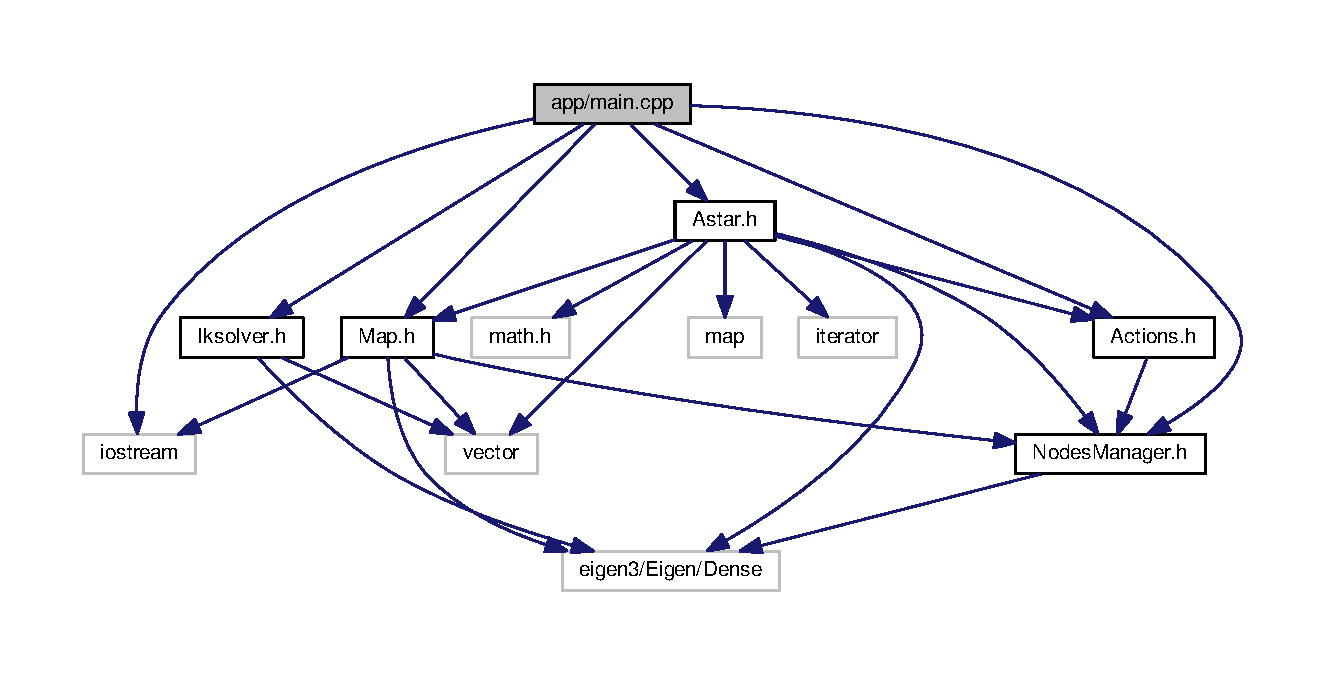
\includegraphics[width=350pt]{main_8cpp__incl}
\end{center}
\end{figure}
\subsection*{Functions}
\begin{DoxyCompactItemize}
\item 
int {\bfseries main} ()\hypertarget{main_8cpp_ae66f6b31b5ad750f1fe042a706a4e3d4}{}\label{main_8cpp_ae66f6b31b5ad750f1fe042a706a4e3d4}

\end{DoxyCompactItemize}


\subsection{Detailed Description}
This is the main file for this project. 

\begin{DoxyCopyright}{Copyright}
M\+IT License
\end{DoxyCopyright}
Implementation (Phase 2) \begin{DoxyAuthor}{Author}
Nischal NJ -\/ Navigator 

Vamshi -\/ Driver 

Raja -\/ Design Keeper 
\end{DoxyAuthor}
\begin{DoxyVersion}{Version}
1.\+0 
\end{DoxyVersion}
\begin{DoxyDate}{Date}
21/10/2019 
\end{DoxyDate}

%--- End generated contents ---

% Index
\backmatter
\newpage
\phantomsection
\clearemptydoublepage
\addcontentsline{toc}{chapter}{Index}
\printindex

\end{document}
